\documentclass[12pt, twoside]{article}
\documentclass[12pt, twoside]{article}
\usepackage[letterpaper, margin=1in, headsep=0.2in]{geometry}
\setlength{\headheight}{0.6in}
%\usepackage[english]{babel}
\usepackage[utf8]{inputenc}
\usepackage{microtype}
\usepackage{amsmath}
\usepackage{amssymb}
%\usepackage{amsfonts}
\usepackage{siunitx} %units in math. eg 20\milli\meter
\usepackage{yhmath} % for arcs, overparenth command
\usepackage{tikz} %graphics
\usetikzlibrary{quotes, angles}
\usepackage{graphicx} %consider setting \graphicspath{{images/}}
\usepackage{parskip} %no paragraph indent
\usepackage{enumitem}
\usepackage{multicol}
\usepackage{venndiagram}

\usepackage{fancyhdr}
\pagestyle{fancy}
\fancyhf{}
\renewcommand{\headrulewidth}{0pt} % disable the underline of the header
\raggedbottom
\hfuzz=2mm %suppresses overfull box warnings

\usepackage{hyperref}
\usepackage{float}

\fancyhead[LE]{\thepage}
\fancyhead[RO]{\thepage \\ First and last name: \hspace{2.5cm} \,\\ Section: \hspace{2.5cm} \,}
\fancyhead[LO]{BECA / Dr. Huson / Regents Prep: Graphs\\* 13 December 2024}

\begin{document}

\subsubsection*{1.16 Do Now Quiz: Graphing inequalities \& times tables}
\begin{enumerate}
\item Graph and label the two inequalities on the grid. 

  \begin{multicols}{2}
    $\displaystyle y \leq \frac{1}{2}x + 2$ \\
    $x + y < 5$
  \end{multicols} \vspace{1cm}

  \begin{center}
  \begin{tikzpicture}[scale=.635]
    \draw [help lines] (-10,-10) grid (10,10);
    \draw [thick, ->] (-10.2,0) -- (10.4,0) node [below right] {$x$};
    \draw [thick, ->] (0,-10.2)--(0,10.4) node [left] {$y$};
  \end{tikzpicture}
  \end{center}

Mark the solution set of the system with a capital ``S''.

\newpage
\subsubsection*{3.OA.7 Fluently perform operations on integers}
\item Perform the calculations.
  \begin{multicols}{2}
    \begin{enumerate}[itemsep=1cm]
      \item $3 \times 4 =$
      \item $2 \times 5 =$
      \item $4 \times 2 =$
      \item $7 \times 3 =$
      \item $2 \times 8 =$
      \item $3 \times 6 =$
    \end{enumerate}
    \end{multicols} \vspace{0.25cm}

    \item Perform the calculations.
    \begin{multicols}{2}
    \begin{enumerate}[itemsep=1cm]
      \item $9 \times 8 =$
      \item $7 \times 6 =$
      \item $8 \times 5 =$
      \item $9 \times 4 =$
      \item $6 \times 7 =$
      \item $7 \times 8 =$
    \end{enumerate}
    \end{multicols} \vspace{0.25cm}

    \item Perform the calculations.
      \begin{multicols}{2}
        \begin{enumerate}[itemsep=0.75cm]
          \item $6 + 3 =$
          \item $5 - 2 =$
          \item $7 + 1 =$
          \item $8 - 4 =$
          \item $9 + 1 =$
          \item $4 - 3 =$
        \end{enumerate}
        \end{multicols} \vspace{0.25cm}

    \item Perform the calculations.
      \begin{multicols}{2}
        \begin{enumerate}[itemsep=0.75cm]
          \item $4 - 5 =$
          \item $-6 - 2 =$
          \item $3 + -7 =$
          \item $8 - (-2) =$
          \item $-2 + 5 =$
          \item $-8 - 6 =$
        \end{enumerate}
        \end{multicols} 

\end{enumerate}
\end{document}